\documentclass[lettersize,journal]{IEEEtran}
\usepackage[UTF8,fontset=windows]{ctex}
\usepackage{amsmath,amsfonts,amssymb}
\usepackage{graphicx}
\usepackage{booktabs}
\usepackage{multirow}
\usepackage{makecell}
\usepackage[caption=false,font=normalsize,labelfont=sf,textfont=sf]{subfig}
\usepackage[hidelinks,unicode]{hyperref}

\hyphenation{op-tical net-works semi-conduc-tor IEEE-Xplore}

\begin{document}

\title{多目标点遍历路径规划协同优化框架——详细实验数据}

\author{论文配套实验数据~\IEEEmembership{（附录材料）}%
\thanks{本文为正稿的详细实验数据附录，正文见 \texttt{paper\_CN.tex}。}}

\markboth{详细实验数据附录}%
{多目标点遍历路径规划——参数敏感性与消融实验}

\maketitle

\begin{abstract}
本文档收录正文中不宜展开的详细实验数据，包括代表性参数敏感性结果表，以及消融实验的平均迭代次数--代价收敛曲线与代价分布图。正文的算法描述、主要结论与其余图表见主论文。
\end{abstract}

\begin{IEEEkeywords}
多目标点遍历，参数敏感性，消融实验，实验数据
\end{IEEEkeywords}

\section{参数敏感性详细结果}
\label{sec:sens}

本节给出与正文参数敏感性分析对应的完整结果表。参数水平依次为$n_{\mathrm{ants}}/q_0/y_{\max}/r_{\mathrm{elite}}/k$；每组配置在Map~1、Map~2与kroB100上各独立运行40次。

\begin{table*}[!t]
\caption{代表性参数敏感性结果}
\label{tab:sens}
\centering
\scriptsize
\setlength{\tabcolsep}{2pt}
\resizebox{\textwidth}{!}{%
\begin{tabular}{llcccc|llcccc}
\toprule
\makecell{Parameter\\level} & Map & Best cost & \makecell{Path\\Mean/std.dev} & \makecell{Run Time\\(ms)} & \makecell{Success rate\\(\%)} & \makecell{Parameter\\level} & Map & Best cost & \makecell{Path\\Mean/std.dev} & \makecell{Run Time\\(ms)} & \makecell{Success rate\\(\%)} \\
\midrule
\multirow{3}{*}{1/3/3/4/2} & Map~1 & \textbf{352.56} & \textbf{352.56}/\textbf{0.00} & \textbf{16.3} & \textbf{100} & \multirow{3}{*}{3/3/4/4/2} & Map~1 & \textbf{352.56} & \textbf{352.56}/\textbf{0.00} & 33.0 & \textbf{100} \\
& Map~2 & \textbf{623.78} & 623.85/0.26 & 241.0 & 92.5 & & Map~2 & \textbf{623.78} & \textbf{623.78}/\textbf{0.00} & 350.5 & \textbf{100} \\
& kroB100 & \textbf{22141.00} & 22143.90/12.80 & \textbf{269.8} & 95 & & kroB100 & \textbf{22141.00} & 22142.45/9.17 & 523.5 & 97.5 \\ \cline{2-6}\cline{8-12}
\multirow{3}{*}{2/3/3/4/2} & Map~1 & \textbf{352.56} & \textbf{352.56}/\textbf{0.00} & 27.0 & \textbf{100} & \multirow{3}{*}{3/3/5/4/2} & Map~1 & \textbf{352.56} & \textbf{352.56}/\textbf{0.00} & 41.8 & \textbf{100} \\
& Map~2 & \textbf{623.78} & 623.83/0.21 & \textbf{232.9} & 95 & & Map~2 & \textbf{623.78} & \textbf{623.78}/\textbf{0.00} & 361.0 & \textbf{100} \\
& kroB100 & \textbf{22141.00} & 22142.97/12.49 & 302.6 & 97.5 & & kroB100 & \textbf{22141.00} & \textbf{22141.00}/\textbf{0.00} & 535.4 & \textbf{100} \\ \cline{2-6}\cline{8-12}
\multirow{3}{*}{3/3/3/4/2} & Map~1 & \textbf{352.56} & \textbf{352.56}/\textbf{0.00} & 38.6 & \textbf{100} & \multirow{3}{*}{3/3/3/1/2} & Map~1 & \textbf{352.56} & \textbf{352.56}/\textbf{0.00} & 49.4 & \textbf{100} \\
& Map~2 & \textbf{623.78} & \textbf{623.78}/\textbf{0.00} & 282.9 & \textbf{100} & & Map~2 & \textbf{623.78} & \textbf{623.78}/\textbf{0.00} & 399.4 & \textbf{100} \\
& kroB100 & \textbf{22141.00} & 22142.45/9.17 & 496.7 & 97.5 & & kroB100 & \textbf{22141.00} & \textbf{22141.00}/\textbf{0.00} & 536.5 & \textbf{100} \\ \cline{2-6}\cline{8-12}
\multirow{3}{*}{4/3/3/4/2} & Map~1 & \textbf{352.56} & \textbf{352.56}/\textbf{0.00} & 41.9 & \textbf{100} & \multirow{3}{*}{3/3/3/2/2} & Map~1 & \textbf{352.56} & \textbf{352.56}/\textbf{0.00} & 46.8 & \textbf{100} \\
& Map~2 & \textbf{623.78} & \textbf{623.78}/\textbf{0.00} & 340.3 & \textbf{100} & & Map~2 & \textbf{623.78} & 623.83/0.21 & 334.0 & 95 \\
& kroB100 & \textbf{22141.00} & 22142.45/9.17 & 486.6 & 97.5 & & kroB100 & \textbf{22141.00} & 22142.45/9.17 & 578.9 & 97.5 \\ \cline{2-6}\cline{8-12}
\multirow{3}{*}{5/3/3/4/2} & Map~1 & \textbf{352.56} & \textbf{352.56}/\textbf{0.00} & 66.6 & \textbf{100} & \multirow{3}{*}{3/3/3/3/2} & Map~1 & \textbf{352.56} & \textbf{352.56}/\textbf{0.00} & 45.3 & \textbf{100} \\
& Map~2 & \textbf{623.78} & \textbf{623.78}/\textbf{0.00} & 429.1 & \textbf{100} & & Map~2 & \textbf{623.78} & \textbf{623.78}/\textbf{0.00} & 331.9 & \textbf{100} \\
& kroB100 & \textbf{22141.00} & 22142.45/9.17 & 643.5 & 97.5 & & kroB100 & \textbf{22141.00} & \textbf{22141.00}/\textbf{0.00} & 450.0 & \textbf{100} \\ \cline{2-6}\cline{8-12}
\multirow{3}{*}{3/1/3/4/2} & Map~1 & \textbf{352.56} & \textbf{352.56}/\textbf{0.00} & 42.0 & \textbf{100} & \multirow{3}{*}{3/3/3/5/2} & Map~1 & \textbf{352.56} & \textbf{352.56}/\textbf{0.00} & 43.5 & \textbf{100} \\
& Map~2 & \textbf{623.78} & \textbf{623.78}/\textbf{0.00} & 515.3 & \textbf{100} & & Map~2 & \textbf{623.78} & 623.80/0.15 & 310.8 & 97.5 \\
& kroB100 & \textbf{22141.00} & \textbf{22141.00}/\textbf{0.00} & 721.9 & \textbf{100} & & kroB100 & \textbf{22141.00} & 22145.35/15.47 & 564.1 & 92.5 \\ \cline{2-6}\cline{8-12}
\multirow{3}{*}{3/2/3/4/2} & Map~1 & \textbf{352.56} & \textbf{352.56}/\textbf{0.00} & 41.7 & \textbf{100} & \multirow{3}{*}{3/3/3/4/1} & Map~1 & \textbf{352.56} & \textbf{352.56}/\textbf{0.00} & 34.7 & \textbf{100} \\
& Map~2 & \textbf{623.78} & 624.01/1.02 & 370.7 & 95 & & Map~2 & \textbf{623.78} & \textbf{623.78}/\textbf{0.00} & 258.5 & \textbf{100} \\
& kroB100 & \textbf{22141.00} & \textbf{22141.00}/\textbf{0.00} & 487.6 & \textbf{100} & & kroB100 & \textbf{22141.00} & 22184.58/40.07 & 765.9 & 42.5 \\ \cline{2-6}\cline{8-12}
\multirow{3}{*}{3/4/3/4/2} & Map~1 & \textbf{352.56} & \textbf{352.56}/\textbf{0.00} & 35.5 & \textbf{100} & \multirow{3}{*}{3/3/3/4/3} & Map~1 & \textbf{352.56} & \textbf{352.56}/\textbf{0.00} & 40.5 & \textbf{100} \\
& Map~2 & \textbf{623.78} & 624.01/1.02 & 357.1 & 95 & & Map~2 & \textbf{623.78} & 623.94/0.87 & 310.6 & 95 \\
& kroB100 & \textbf{22141.00} & 22148.78/21.05 & 441.3 & 87.5 & & kroB100 & \textbf{22141.00} & 22143.90/12.80 & 508.4 & 95 \\ \cline{2-6}\cline{8-12}
\multirow{3}{*}{3/5/3/4/2} & Map~1 & \textbf{352.56} & \textbf{352.56}/\textbf{0.00} & 37.6 & \textbf{100} & \multirow{3}{*}{3/3/3/4/4} & Map~1 & \textbf{352.56} & \textbf{352.56}/\textbf{0.00} & 34.9 & \textbf{100} \\
& Map~2 & \textbf{623.78} & 624.72/1.82 & 302.2 & 70 & & Map~2 & \textbf{623.78} & \textbf{623.78}/\textbf{0.00} & 383.4 & \textbf{100} \\
& kroB100 & \textbf{22141.00} & 22178.55/45.78 & 409.3 & 57.5 & & kroB100 & \textbf{22141.00} & 22142.45/9.17 & 519.5 & 97.5 \\ \cline{2-6}\cline{8-12}
\multirow{3}{*}{3/3/1/4/2} & Map~1 & \textbf{352.56} & \textbf{352.56}/\textbf{0.00} & 40.4 & \textbf{100} & \multirow{3}{*}{3/3/3/4/5} & Map~1 & \textbf{352.56} & \textbf{352.56}/\textbf{0.00} & 43.7 & \textbf{100} \\
& Map~2 & \textbf{623.78} & 624.47/1.30 & 372.0 & 62.5 & & Map~2 & \textbf{623.78} & \textbf{623.78}/\textbf{0.00} & 356.7 & \textbf{100} \\
& kroB100 & \textbf{22141.00} & 22149.10/25.05 & 486.7 & 90 & & kroB100 & \textbf{22141.00} & 22145.35/15.47 & 505.4 & 92.5 \\ \cline{2-6}\cline{8-12}
\multirow{3}{*}{3/3/2/4/2} & Map~1 & \textbf{352.56} & \textbf{352.56}/\textbf{0.00} & 38.3 & \textbf{100} & & & & & & \\
& Map~2 & \textbf{623.78} & 624.00/0.47 & 343.8 & 80 & & & & & & \\
& kroB100 & \textbf{22141.00} & \textbf{22141.00}/\textbf{0.00} & 424.2 & \textbf{100} & & & & & & \\
\bottomrule
\end{tabular}
}
\end{table*}



\section{消融实验详细图示}
\label{sec:abl}

本节补充正文消融分析所引用的收敛曲线与代价分布图，便于读者对照正文结论进行复核。

\begin{figure*}[!t]

\centering
\subfloat[Map~1]{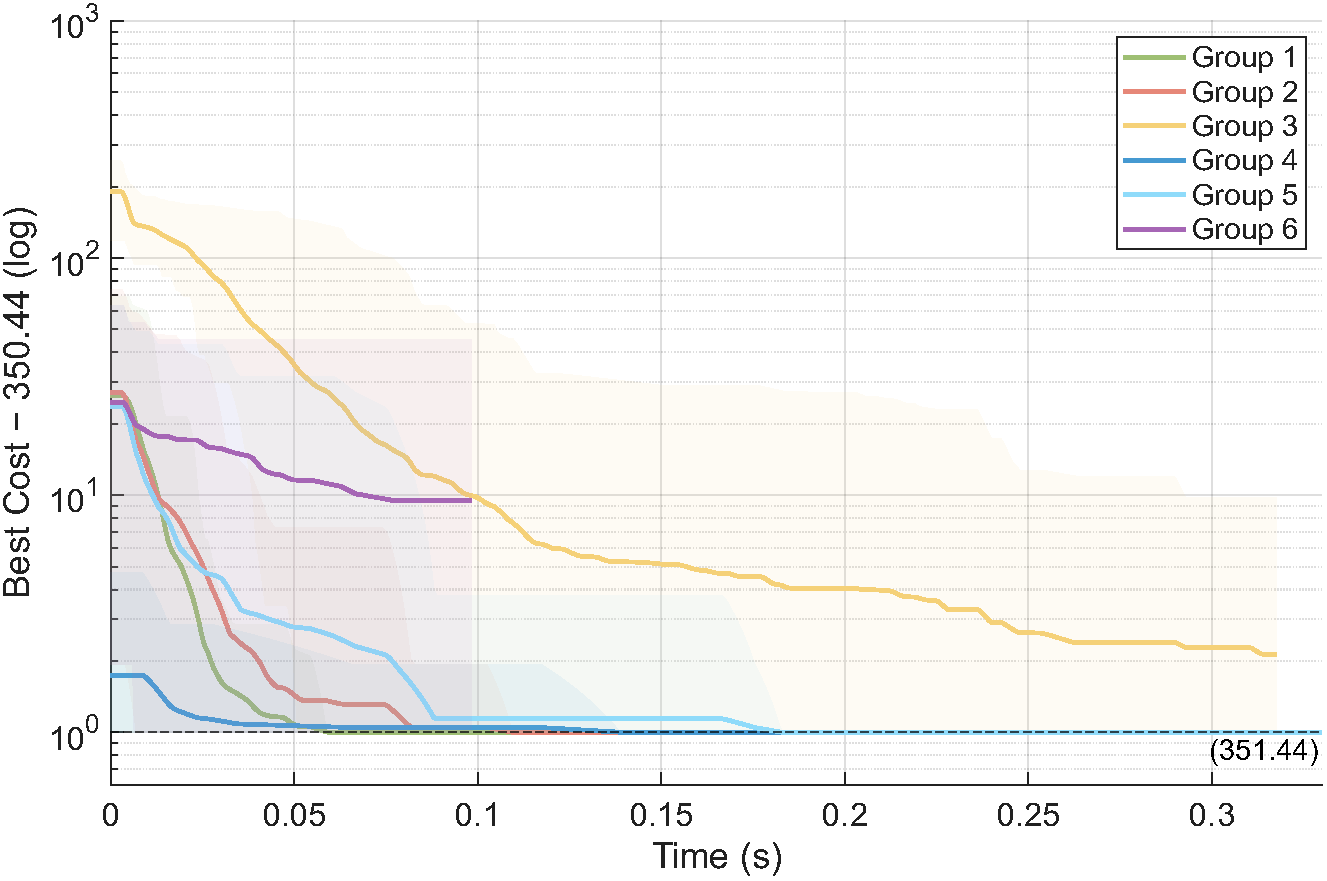
\includegraphics[width=0.3\textwidth]{../figures/Ablation_Conv_Map1}\label{fig:abl_conv_a}}\hfil
\subfloat[Map~2]{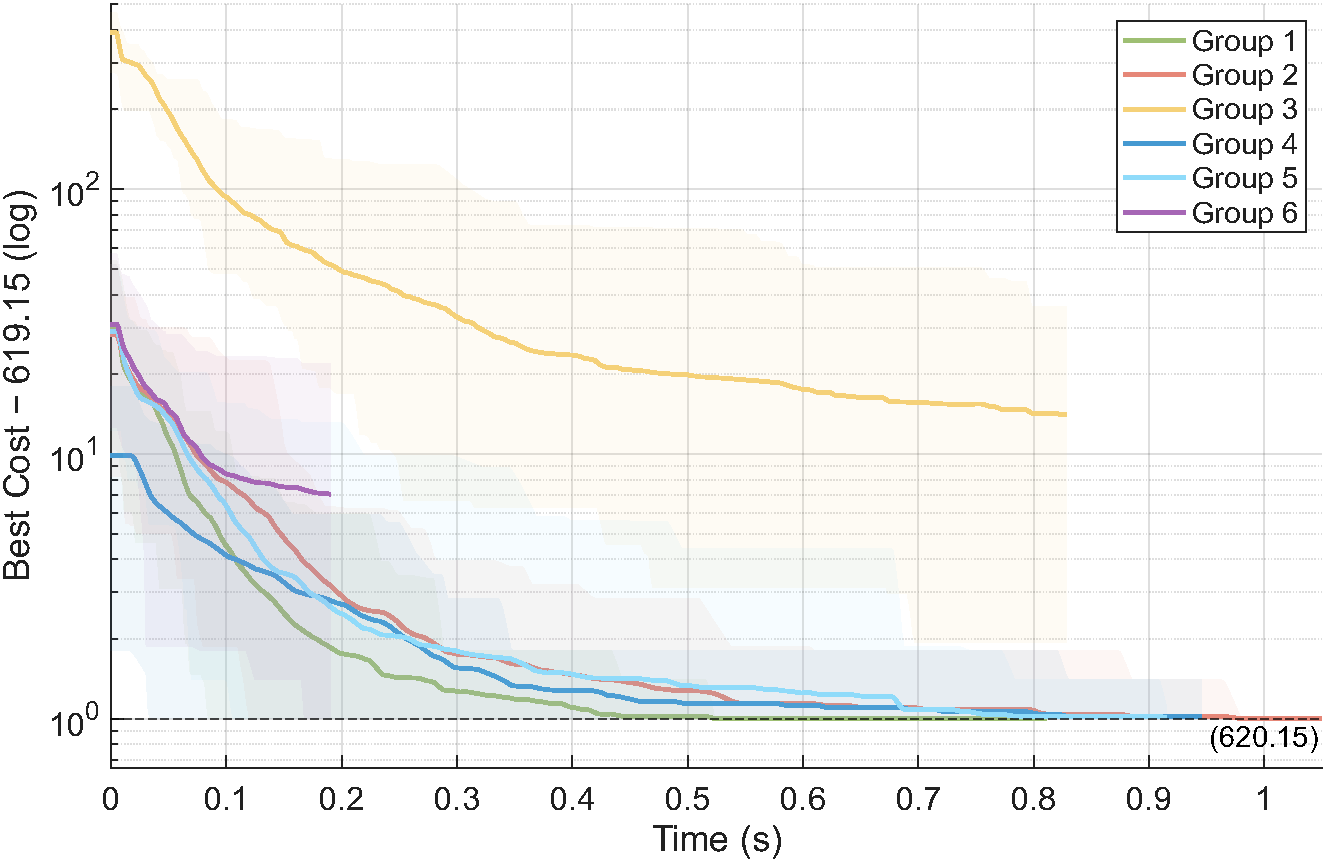
\includegraphics[width=0.3\textwidth]{../figures/Ablation_Conv_Map2}\label{fig:abl_conv_b}}\hfil
\subfloat[kroB100]{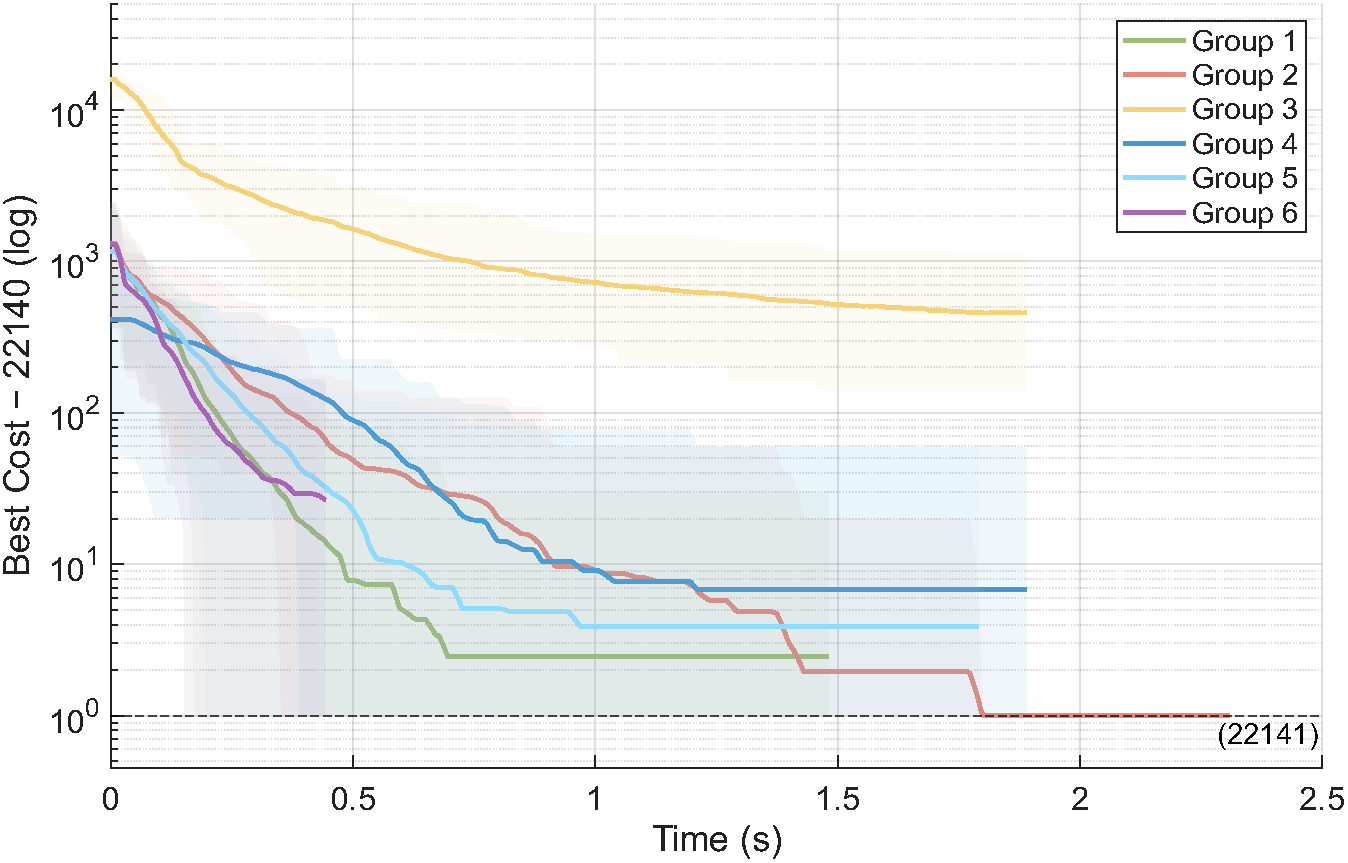
\includegraphics[width=0.3\textwidth]{../figures/Ablation_Conv_kroB100}\label{fig:abl_conv_c}}
\caption{六个消融组在三张地图上40次运行的平均迭代次数-代价收敛曲线。}
\label{fig:abl_conv}
\end{figure*}


\begin{figure*}[!t]

\centering
\subfloat[Map~1]{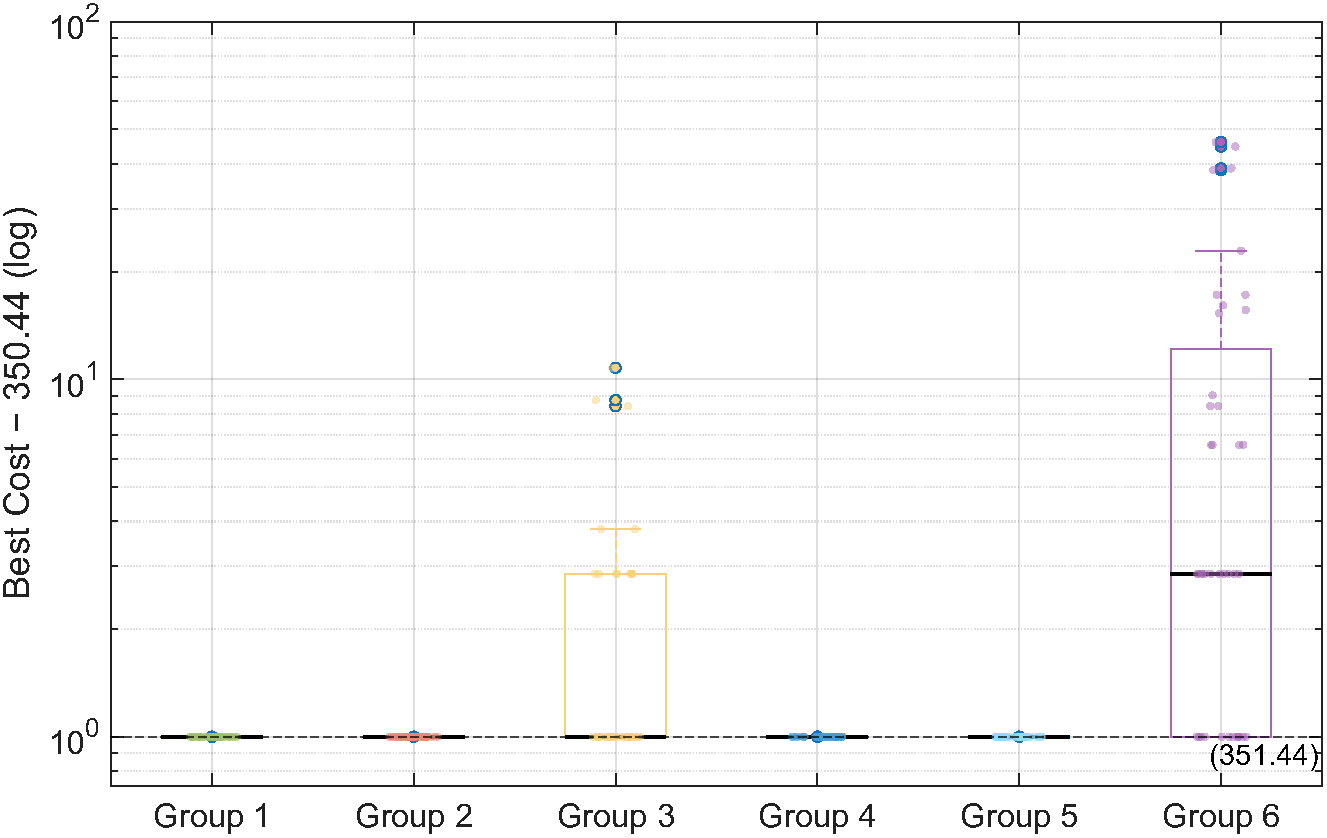
\includegraphics[width=0.3\textwidth]{../figures/Ablation_Box_Map1}}\hfil
\subfloat[Map~2]{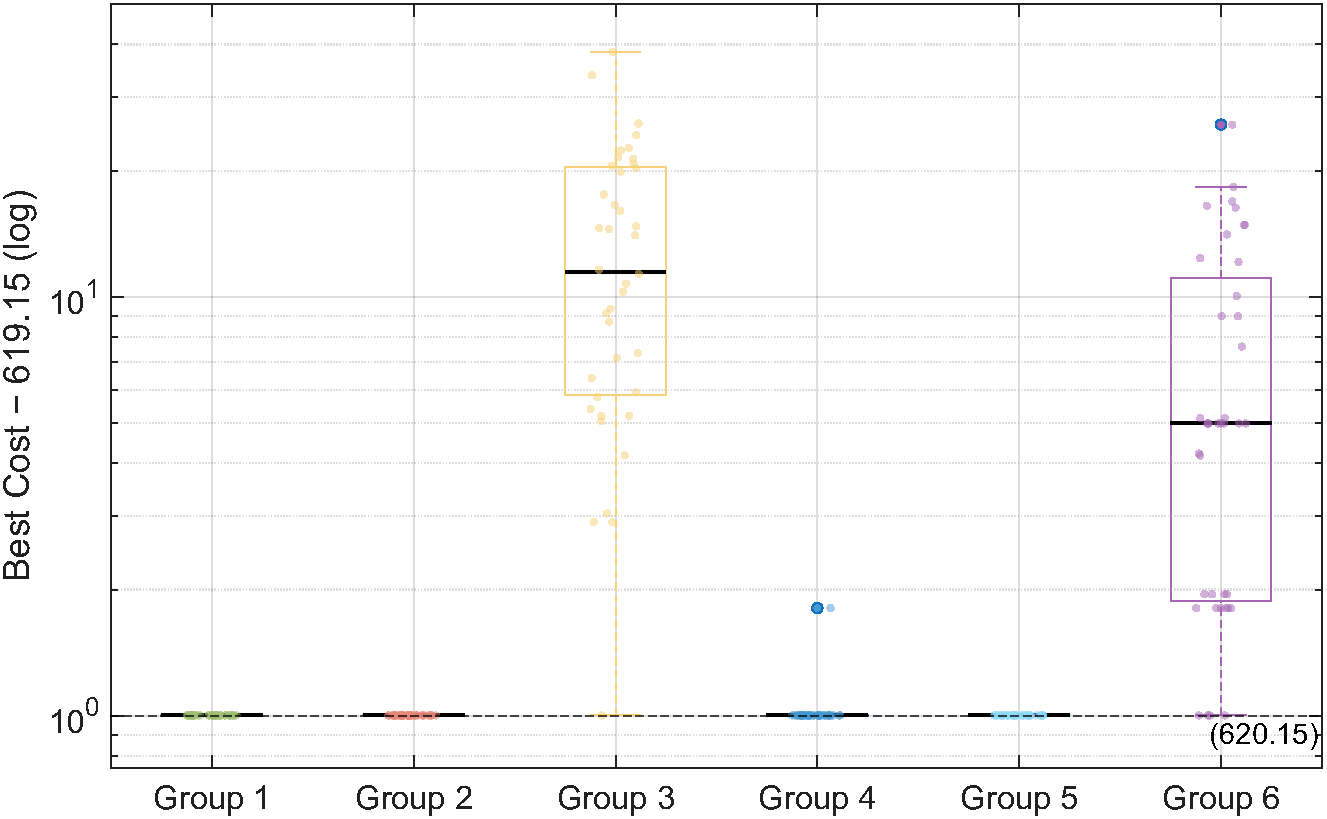
\includegraphics[width=0.3\textwidth]{../figures/Ablation_Box_Map2}}\hfil
\subfloat[kroB100]{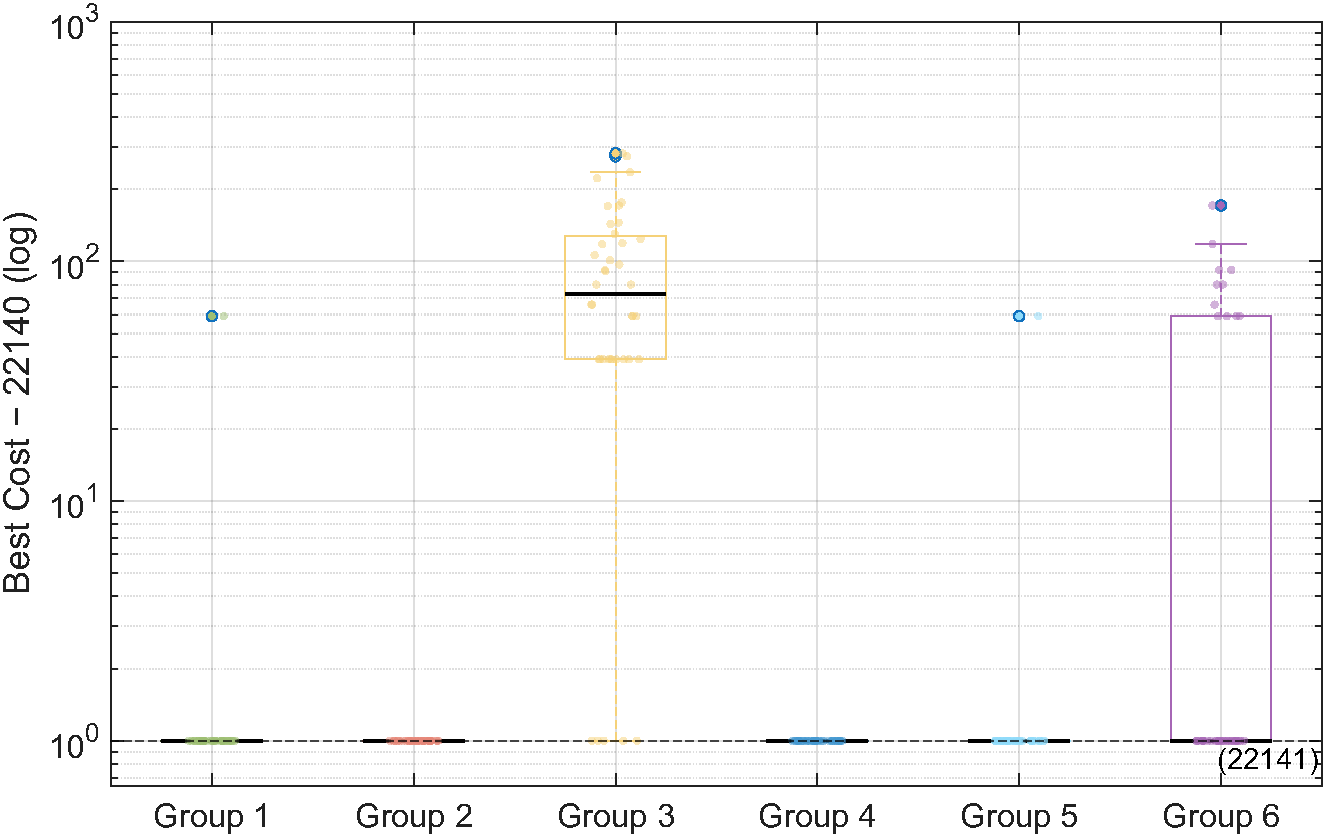
\includegraphics[width=0.3\textwidth]{../figures/Ablation_Box_kroB100}}
\caption{六个消融组在三张地图上40次运行的代价分布。}
\label{fig:abl_box}
\end{figure*}



\vfill
\end{document}
